\documentclass[12pt]{article}

\usepackage[margin=1in]{geometry}

\usepackage{graphicx}
\graphicspath{ {./plots/} }
\usepackage{mathtools}
\usepackage{derivative}

\title{Self-supervised learning with autoencoders}
\author{Jia Geng Chang }
\date{December 2021}


\begin{document}

\maketitle

This is a classical autoencoder for intended for CPU training, that is written in optimized code using C. 

\section{Encoding a 8-bit one-hot vector with 3 bits}

I trained a multi-layer perceptron to encode with 3 units a one-hot encoded vector of length 8.  e.g. \begin{pmatrix}0 & 0 & 0 & 0 & 0 & 0 & 1 & 0\end{pmatrix} represents the decimal digit 7 and \begin{pmatrix}0 & 0 & 0 & 4 & 0 & 0 & 0 & 0\end{pmatrix} represents the decimal digit 4. Because only one value can be 1, there are only 8 such vectors corresponding to the rows of a 8x8 identity matrix — a relatively easy pattern for the network to learn to encode and decode.

Here are the hyperparameters of the autoencoder:
\begin{table}[htbp]
    \centering
    \begin{tabular}{|c|c|c|}
    \hline
    activation function & sigmoid & $\sigma(x) = \frac{1}{1 + exp(-x}$\\
    \hline
    loss function & binary cross-entropy & *equation below\\
    \hline
    optimizer & classical momentum & m=0-0.9 \\
    \hline
    learning rate & min 0.01 & max 1.0 \\
    \hline
    weights & random uniform initialization & Between -0.1 and 0.1 \\
    \hline
    
    \end{tabular}
    \caption{Network architecture}
    \label{tab:my_label}
\end{table}

Binary cross-entropy loss is:
\begin{equation}
    -\frac{1}{N}\,\sum_{k=1}^{N}\,t_{k}\,log(p_{k}) + (1-t_{k}))\,(log(1-p_{k}))
\end{equation}
where $\mathbf{t}$ is the target one-hot encoded vector, and $\mathbf{p}$ is the output layer activation which is a probability vector, and $N$ is 8 in our case. The derivatives of loss with respect to weights worked out to be:
\begin{equation}
    \pdv{E}{W_{jk}} = -\frac{1}{N}\,(\frac{t_{k}}{z_{k}}-\frac{1-t_{k}}{1-z_{k}})\: g'(x_{k})\: z_{j} = \delta_{k}z_{j}
\end{equation}
for the weights between hidden and output units and 
\begin{equation}
    \pdv{E}{W_{ij}} = -\frac{1}{N} \sum\limits_{k=1}^{N} \: (\frac{t_{k}}{z_{k}}-\frac{1-t_{k}}{1-z_{k}})\: g'(x_{k}) \: w_{jk} \: g'(x_{j}) \: z_{i} = \delta_{j}z_{i}
\end{equation}
for the weights between input and hidden units. The derivative $g'$ of the sigmoid function $g$ is $g' = g(1-g)$.

\section{Training results}

\begin{figure}[htbp]
    \centering
    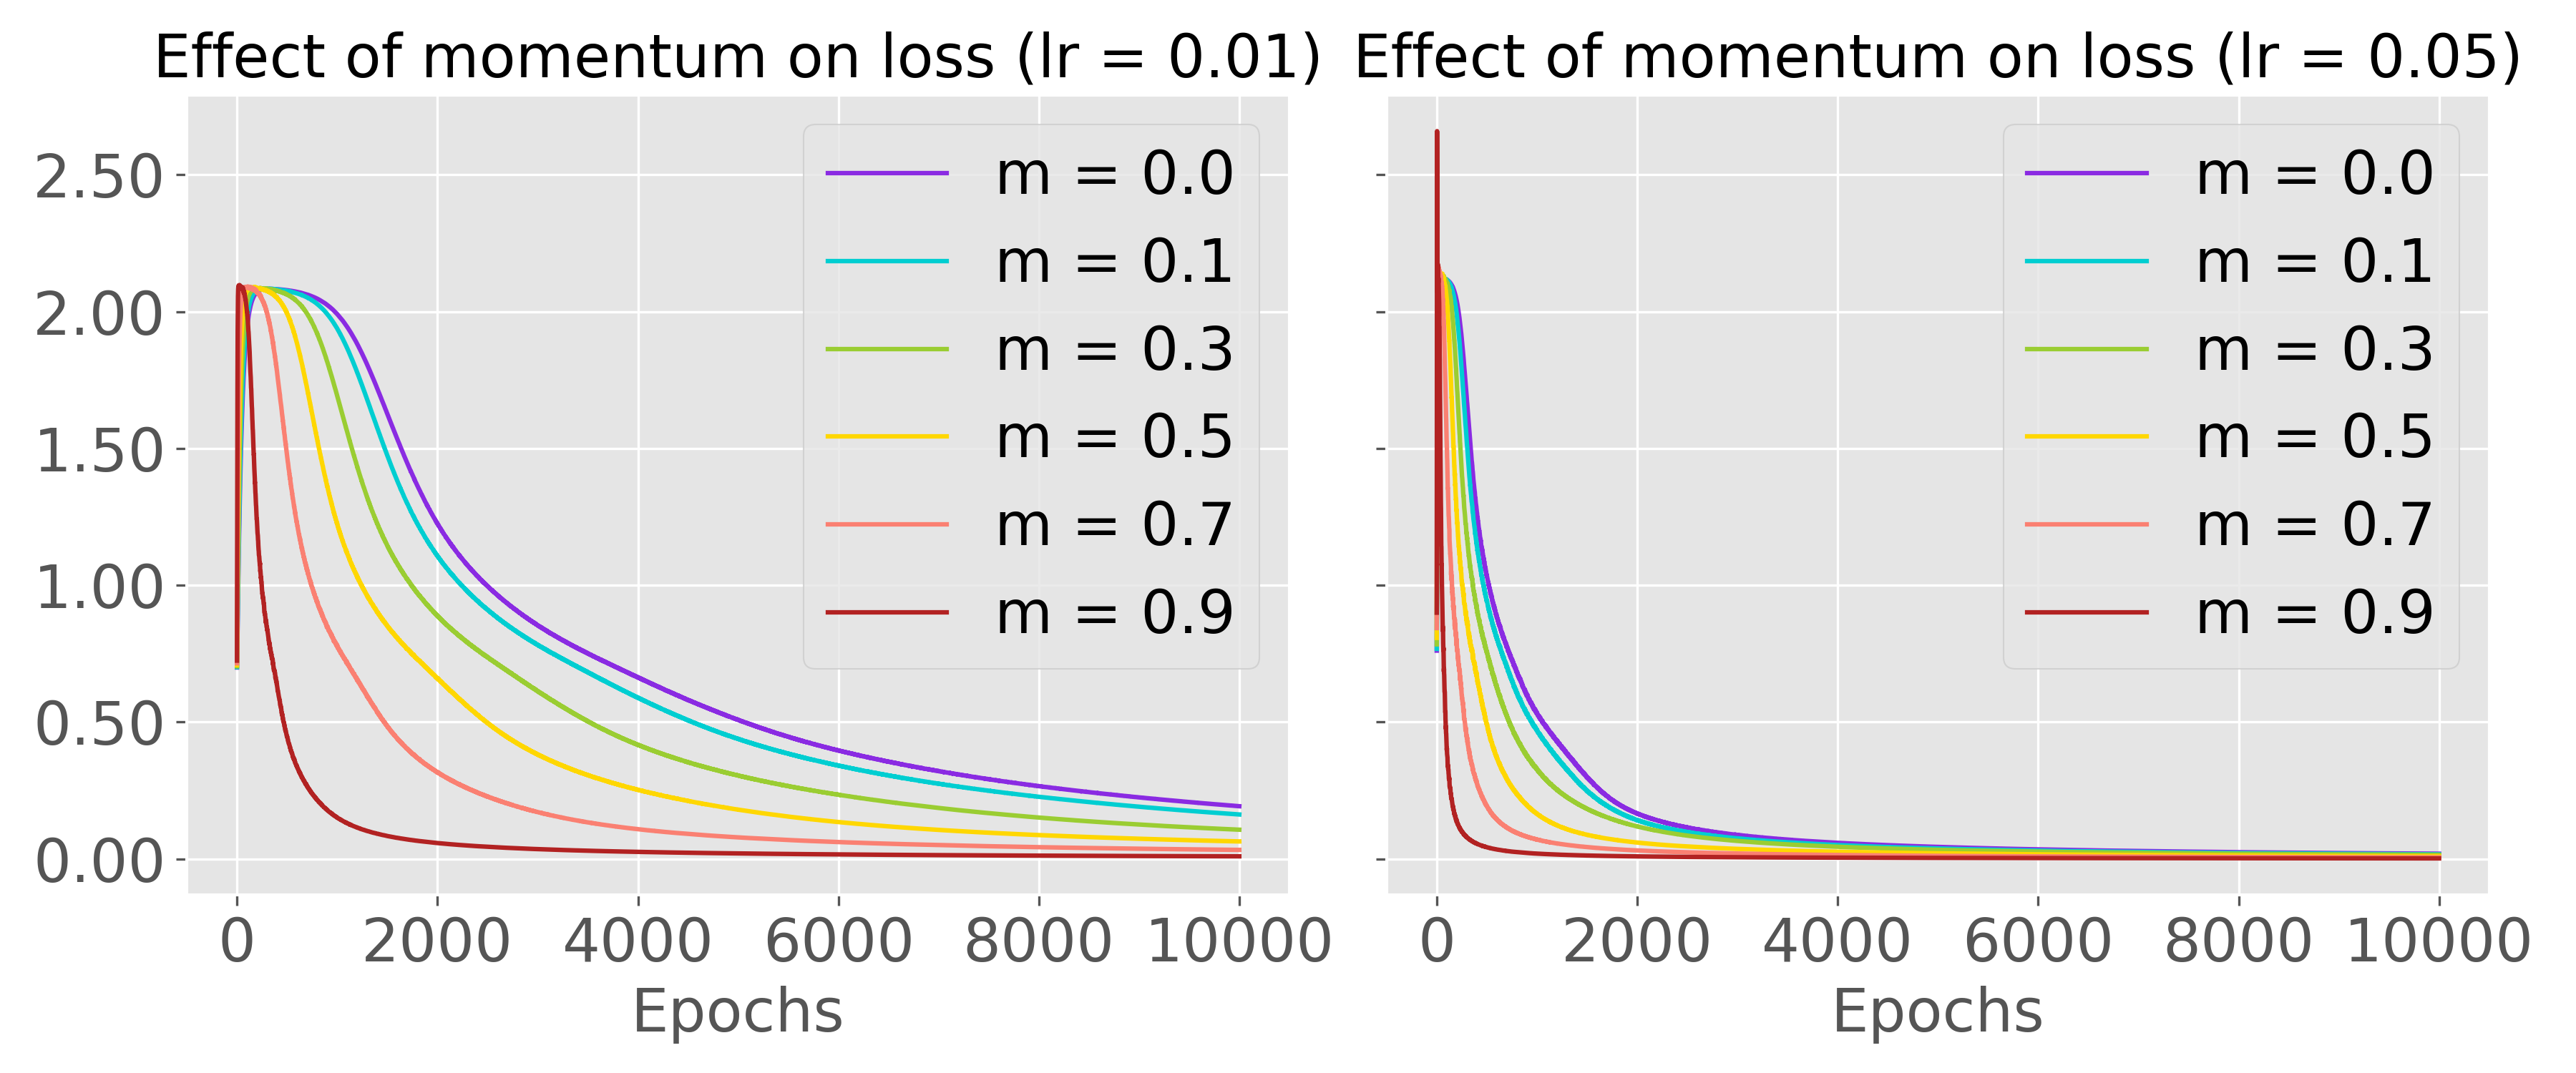
\includegraphics[width=12cm, height=5cm]{mlp_m}
    \caption{With learning rate held constant, momentum speeds up learning}
    \label{fig:mlp_momentum}
\end{figure}

With standard gradient descent, training was slow, even at high learning rates of up to 10. Thus, I added a momentum term involving the previous time step as a modification to vanilla gradient descent. The weight update heuristic at epoch $t$ becomes:

\begin{equation}
    \Delta W_{ij}(t) = -\eta \, \pdv{E}{W_{ij}} + m \,\Delta W_{ij}(t-1)
\end{equation}

for a pair of connected neurons $i$ and $j$, and m is scalar that practitioners suggest to be kept between 0 and 1. The result in training with varying $m$, for two different learning rates (lr = 0.01 and lr = 0.05) is shown in figure \ref{fig:mlp_momentum}. 


From \ref{fig:mlp_momentum}, we can see that adding momentum speeds up training greatly. What is happening is that the magnitude of $\Delta W_{ij}(t)$ is increasing by a factor of close to $1+m$ as a function of $t$, because each time $\nabla E(t)$ is in a similar direction as $\nabla E(t-1)$.

\section{How 8-3-8 autoencoder learns input representation}
How is the network learning to encode input vectors? We look at the final state of the weights for the best network to see what is happening.

\begin{figure}[htbp]
    \centering
    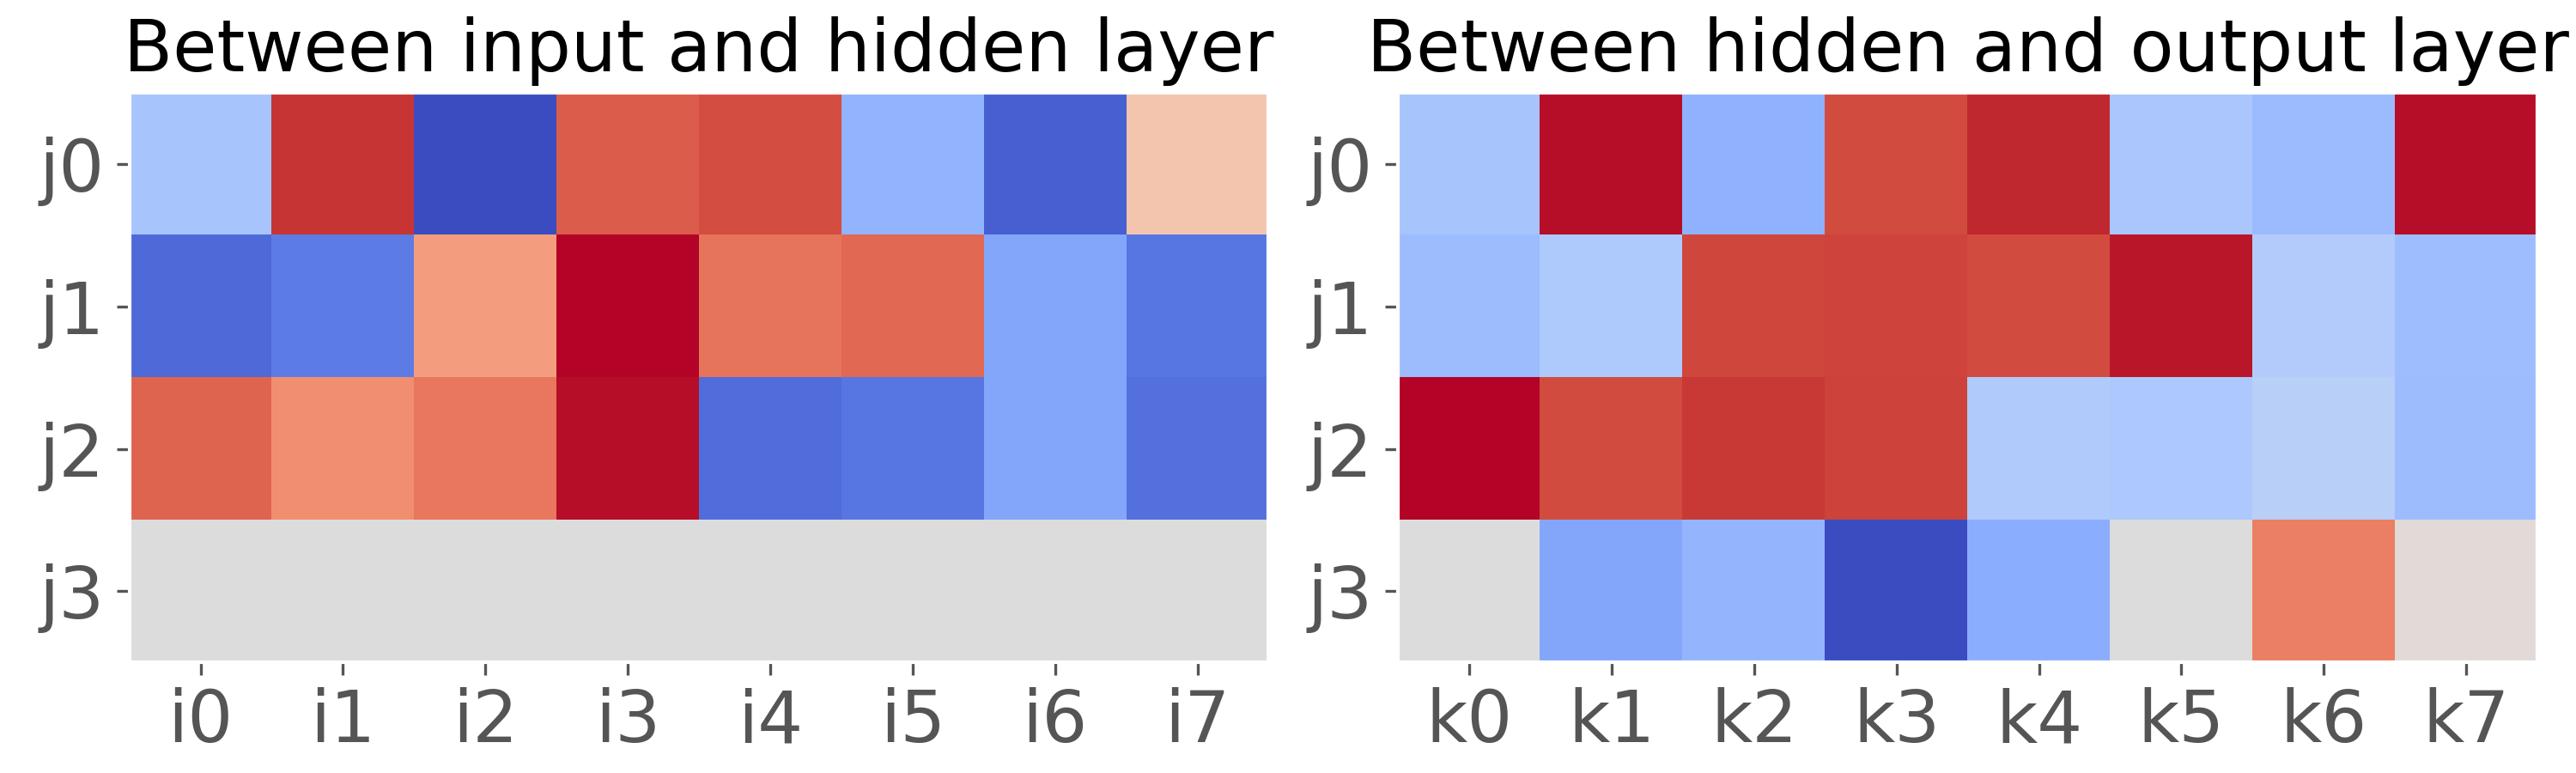
\includegraphics[width=10cm, height=3cm]{mlp_w}
    \caption{The network learns to mirror weights between the three layers}
    \label{fig:mlp_w}
\end{figure}

Without loss of generality, what the network has learned is to match the signs between mirrored pairs of weights ${W_{nj},\; W_{jn} \; \forall \; n \in [0,7], \; j \in [0,2]}$. For example, if $\mathbf{t}$ is \begin{pmatrix}1 & 0 & ... & 0\end{pmatrix}, then only $j_0$ and $k_0$ will fire, producing a large positive activation in $k_0$ because $W_{i0,j0}$ and $W_{j0,k0}$ have the same sign (does not matter whether positive or negative). The two other hidden units also have synergistic weights entering/leaving them, but they will stay silent because the inputs into those units is 0. 

\section{Encoding a 16-bit one-hot vector with 3 bits}

\begin{figure}[htbp]
    \centering
    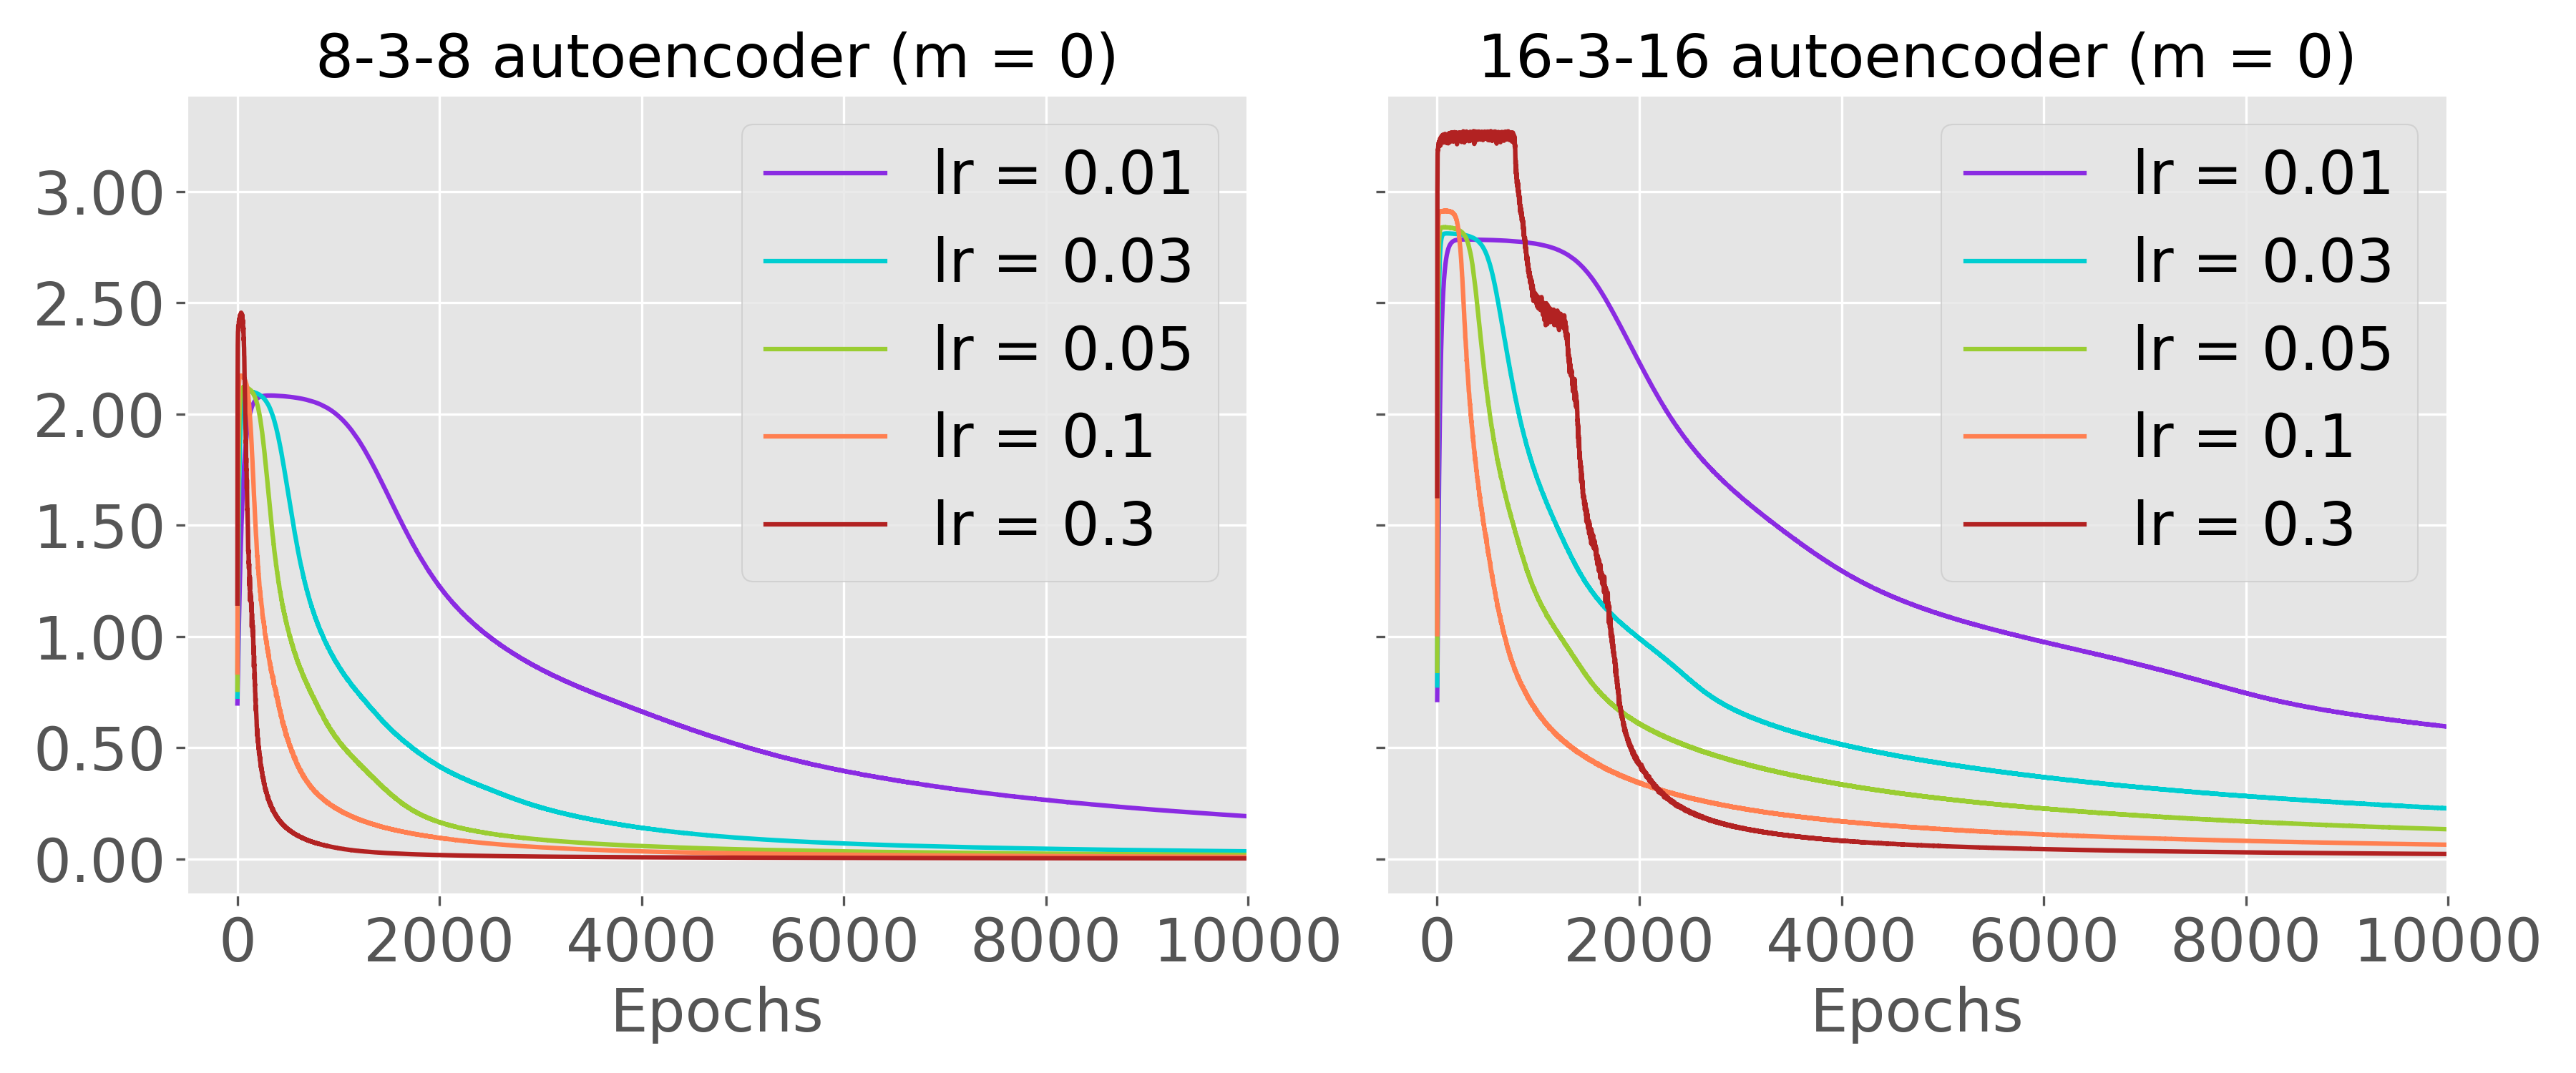
\includegraphics[width=12cm, height=5cm]{mlp_8_16}
    \caption{The 16-3-16 multi-layer perceptron trains slower across learning rates. Vertical axis is binary cross-entropy loss.}
    \label{fig:mlp_8_16}
\end{figure}
Is it possible to be even more efficient and encode a one-hot vector \textit{twice} the size as our previous vector, with 3 hidden units? If each hidden unit can represent 3 activation states, then we can encode up to a one-hot vector of length $3^n = 3^3 = 27$. As we are using a sigmoid activation, the three activation states are naturally 0, 0.5, and 1, requiring asymptotic input values of $-\infty$, 0, and $\infty$ at each hidden unit. While our loss will again never reach 0, it is theoretically possible to train such a network.

In figure \ref{fig:mlp_8_16}, I trained a multi-layer perceptron to encode with 3 units a one-hot encoded vector of length \textbf{16}. Training is slower, because there are more weights to adjust, but binary cross-entropy is reduced to a similar extent after around 10000 epochs. 

\section{How 16-3-16 autoencoder learns input representation}

\begin{figure}
    \centering
    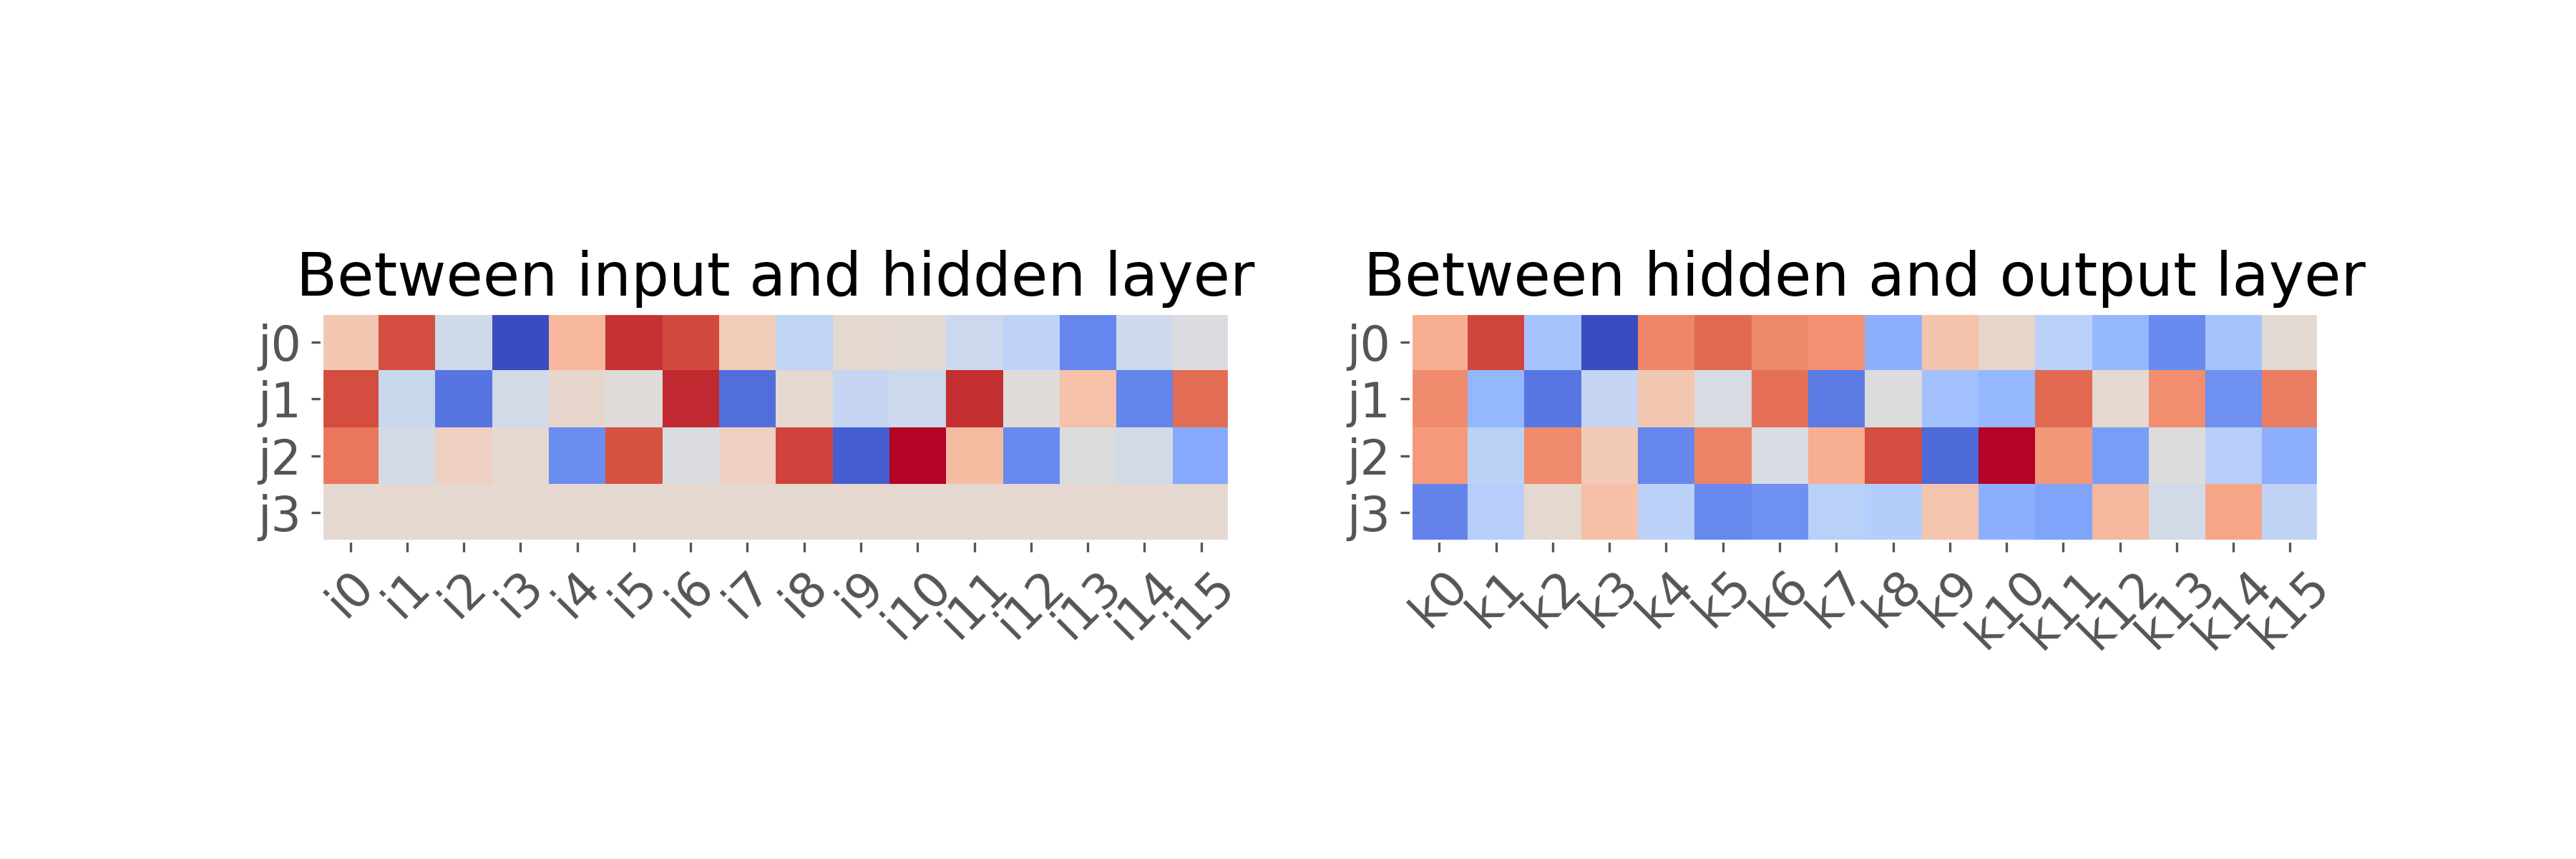
\includegraphics[height=3cm]{mlp16_w}
    \caption{Weights are again mirrored, and every hidden unit has 3 states - red, white and blue}
    \label{fig:mlp16_w}
\end{figure}

Visualizing the weight matrices in figure \ref{fig:mlp16_w}, we see that the network is again solving the problem by mirroring the sign of the weights. Additionally, it mirrors the relative magnitude of the weights. This time, each hidden node has three states, as the mirrored incoming and outgoing weights are in one of negative (blue), zero (off-white), and positive (red). The connections entering output node 14 (k14) look all negative, but this is offset by the positive bias ($W_{j3,k14}$). Again, the bias in the input layer is not doing much (it cannot be any other value than 0 otherwise non-1 units will fire), but the bias in the hidden layer is helping to adjust the median weight to zero.

\section{Code availability}
The code for the 8-unit multi-layer perceptron is available as \textbf{\texttt{testmlp.c}}, and the code for the 16-unit multi-layer perceptron is found in \textbf{\texttt{testmlp16.c}}. I also include a \texttt{utils.c} definitions file for simple matrix operations required (e.g., dot product, hadamard product, and scalar operations). The \textbf{\texttt{output}} directory contains the \texttt{.csv} files used to generate the plots. Jupyter notebooks for generating the plots are also included as \texttt{.ipynb} files, and the \texttt{.png} files are found in \texttt{plots}.


\end{document}